Считывающая электроника жидкаргоновых калориметров детектора ATLAS имеет сложную структуру, но в самом верхнем уровне её можно разделить на 2 части: фронтенд и бэкенд(или как её ещё называют, задетекторная электроника). На рис. \ref{fig:read_electronics} изображена общая схема устройства считывающей электроники системы жидкоаргоновы калориметров.
\begin{figure}[ht]
    \centering
    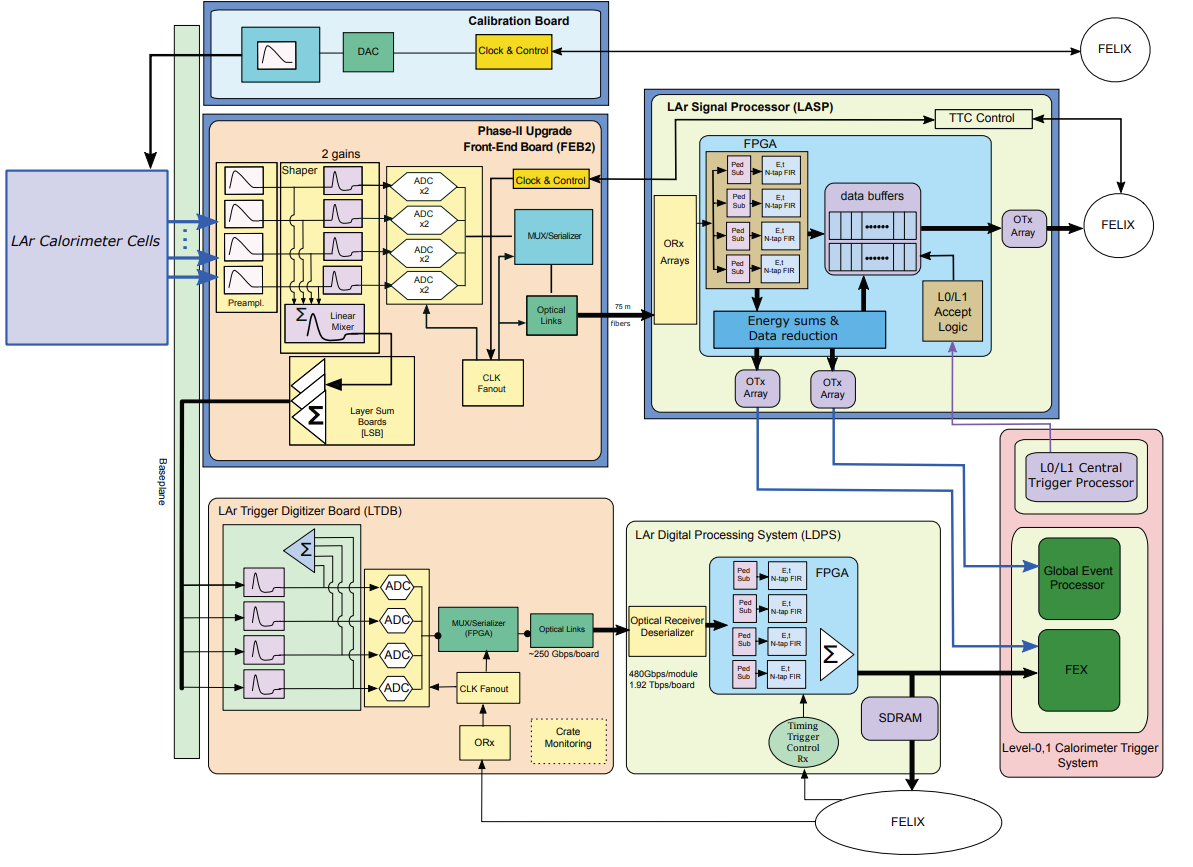
\includegraphics[width=\linewidth]{read_electronics.png}
    \caption{Схема считывающей электроники жидкоаргоновых калориметров ATLAS}
    \label{fig:read_electronics}
\end{figure}\par
Фронтенд часть располагается в непосредственной близости с ускорителем, поэтому на неё налагаются определённые требования по радиационной стойкости и отказоустойчивости. В рамках второй фазы обновления электроники на детектор будут установлены новые платы считывания FEB2(FEB -- Front-End Board), а также платы калибровки.\par
Задетекторная часть удалена от радиационной зоны и принимает оцифрованные данные с фронтенда через оптические каналы связи. Именно в этой части выполняется цифровая фильтрация сигналов по каждой ячейке калориметра, их буферихация до появления сигнала триггерной системы и передача соответствующих данных в систему сбора данных DAQ (Data Acquisition).\par

\subsubsection{Модуль FEB2}
Платы FEB2 принимают сигналы от калориметрических ячеек и выполняют их аналоговую обработку, включая усиление, формирование и разделение на две перекрывающиеся шкалы линейного усиления. Обе шкалы усиления оцифровываются при помощи аналого-цифрового преобразователя (АЦП), после чего цифровые сигналы сериализуются и отправляются через оптический канал связи. Для этого используется несколько специализированных интегральных микросхем, а также системы управления и синхронизации. Оцифровка данных производится на частоте 40 МГц, равной частоте столкновения частиц. Каждая плата FEB2 способна обрабатывать 128 калориметрических каналов, а для считывания всей системы жидкоаргоновых калориметров требуется 1524 таких устройства.\par
Аналоговая обработка данных выполняется в 2 этапа. На первом этапе выполняется усиление сигналов калориметра, которые имеют динамический диапазон до 16 бит, с помощью специального предусилителя. Второй каскад -- формирователь, который преследует две цели. Во-первых, он необходим для преобразования выходного сигнала схемы предварительного усилителя в дифференциальный выходной сигнал с несколькими коэффициентами усиления, а во-вторых, для получения по крайней мере одного этапа формирования в соответствии с требованиями к обработке сигнала. При необходимости могут быть добавлены несколько эквивалентных этапов формирования с минимальными затратами энергии. Как предусилитель, так и формирователь реализуются в одной специализированной интегральной микросхеме LAPAS (Liquid Argon Preamplifier And Shaper \parencite{lapas}), способной обрабатывать 4 либо 8 калориметрических сигналов.\par
В дополнение к усилению и формированию сигнала необходимы периферийные схемы, такие как генератор тестовых импульсов, схема смещения, датчик температуры, а также регистры конфигурации всего модуля.\par
Далее аналоговый сигнал от каждой калориметрической ячейки оцифровывается с частотой 40 МГц, синхронно с частотой соударения пучков в Большом Адронном коллайдере. Для охвата 16-битного динамического диапазона сигнал оцифровывается с двумя шкалами усиления с помощью 14-битных АЦП. Затем каждый выходной сигнал АЦП форматируется в 16-битное слово и сериализуется со скоростью передачи данных 640 Мбит/с. Каждое такое слово помимо 14 бит данных АЦП содержит бит чётности для обеспечения проверки ошибок. Учитывая, что каждая плата FEB2 обрабатывает 128 калориметрических каналов, результирующая скорость передачи данных составляет 163,84 Гбит/с (256 потоков по 640 Мбит/с каждый). Для передачи оцифрованных данных используются специально разработанные радиационно-стойкие трансивер и лазер lpGBT (low power GigaBit Tranceiver \parencite{lpgbt}). \par
Для реализации корректной синхронизации данных калориметра в модуле FEB2 предусмотрена генерация идентификатора соударения пучков (BCID -- Bunch Crossing Identifier). Данный идентификатор представлен в виде 12-битного счётчика, который инкриминируется с частотой возникновения событий в коллайдере и сбрасывается после каждого завершения цикла столкновений пучков частиц на орбите. Значение BCID, как и данные АЦП, сериализуются и передаются в систему задетекторной электроники через оптический канал.\par
Кроме основного тракта данных в модуле FEB2 присутствует подсистема, которая обеспечивает формирование входных данных для платы LTDB (LAr Trigger Digitizer Board \parencite{ltdb}). Данная плата обрабатывает аналоговые суммы сигналов для максимально быстрого принятия решения триггерной системы, но с более грубой детализацией, чем обеспечивается основным считыванием. Модуль FEB2 имеет набор сумматоров, которые формируют требуемые аналоговые сигналы сумм по соседним ячейкам калориметра.\par


\subsubsection{Система подготовки данных для триггера}
В целях получения как можно более быстрого решения триггерной системы, пусть даже и менее точного, в считывающей электронике жидкоаргоновых калориметров ATLAS предусмотрена система подготовки и передачи энергетических сумм по частям детектора в триггер. Такие сигналы генерируются в модуле FEB2, после чего в аналоговом виде отправляются на плату оцифровки триггера LTDB. Каждая такая плата способна обрабатывать до 320 сигналов, оцифровывая их с помощью 80 12-битных четырёхканальных АЦП \parencite{ltdb}. Далее эти значения передаются на двадцать трансиверов lpGBT, которые формируют 40 выходных потоков с объёмом данных 5,12 Гбит/с каждый для их отправки по волоконно-оптическим каналом связи в систему LDPS (LAr Digital Processing System). Всего в системе считывающей электроники предусмотрено 124 модуля LTDB, которые, соответственно, суммарно генерируют поток данных со скоростью примерно 25 Тбит/с.\par
Управление и мониторинг системы оцифровки данных триггера осуществляется по каналам связи 5 Гбит/с, подключенным через интерфейс обмена данными между фронтенд подключениями FELIX (Front-End LInks eXchange \parencite{felix}) в систему сбора данных и триггера ATLAS TDAQ (Trigger and Data Acquisition \parencite{tdaq}).\par
Обработанные в LTDB данные затем передаются в систему цифровой обработки LDPS, которая преобразует измерения АЦП в откалиброванные значения энергии в режиме реального времени. Система построена с использованием мезонинных плат расширений AMC (Advanced Mezzanine Card), которые выполняют точное восстановление энергии и определение настоящего времени столкновения пучков. Для реализации данных функций в платах расширения применяются программируемые логические интегральные схемы Altera Arria-10.\par


\subsubsection{Калибровочная система}
Важной частью фронтенд электроники является калибровочная система. С помощью специальных плат реализуется подача точных калибровочных сигналов непосредственно на ячейки жидкоаргонового калориметра. Форма калибровочного сигнала максимально приближена к импульсу ионизации, генерируемому электромагнитным ливнем в детекторе. В силу того, что получить истинно треугольный сигнал с помощью электронной схемы достаточно трудно, первоначально создаётся экспоненциальный импульс, у которого обрезается область затухания для максимального приближения к желаемой треугольной форме, по крайней мере, в начальной части импульса. Для компенсации остаточной разницы в форме между физическим импульсом ионизации и калибровочным сигналом производится непосредственное измерение свойств последнего для их учёта в процедуре калибровки.\par


